\chapter{Introduction}\label{chap:introduction}

The SafeScript project addresses the critical need for enhanced security in software development by developing an advanced tool that identifies 
security vulnerabilities within software projects. This project aims to provide users with comprehensive capabilities to log in, create, and manage projects, 
and scan code repositories or Python source files for various vulnerabilities. The system employs sophisticated machine learning models to detect 
potential security issues and generates detailed reports. Additionally, users can rescan their code after making necessary fixes to ensure that security 
improvements are effectively implemented.

The project encompasses several functional requirements. 
First, it includes a user authentication feature where users must log in with a username and password to access the system, ensuring secure access. 
Second, it allows for project creation, enabling users to create new projects by providing a name and selecting a code repository or uploading a 
Python source code file. 
Third, repository management lets users specify the source of the code, either via a repository link or direct file upload. 
Fourth, the code retrieval function automates the process of fetching the code from the specified repository or processing the uploaded file. 
Fifth, data conversion converts the retrieved code into word2vec (w2v) format for subsequent vulnerability analysis. 
Sixth, vulnerability detection utilizes pre-trained machine learning models (LSTM, ChatGPT API \cite{chatgpt}) to identify vulnerabilities in the code. 
Seventh, report generation produces a comprehensive report detailing detected vulnerabilities, their severity, and recommendations for remediation. 
Eighth, the rescan capability allows users to rescan their code post-fix to confirm that vulnerabilities have been addressed. 
Lastly, the system supports the detection of specific types of vulnerabilities, including XSS (Cross-Site Scripting), Path Disclosure, Remote 
Code Execution, and Command Injection.

The technical architecture of the SafeScript system comprises several key components. 
The user interface (UI) includes a login page, a dashboard for project management, and options for report viewing and rescanning. 
The backend includes services for authentication, project management, code retrieval, vulnerability detection, and report generation. 
The database stores user credentials, project details, and scanning results and reports. 
The system also incorporates pre-trained machine learning models (LSTM and ChatGPT API) for vulnerability detection.

The workflow of the SafeScript system involves several steps. Initially, the user logs in using credentials. 
The user then creates a new project and selects the source of the code. 
The system fetches the code from the repository or processes the uploaded file. 
The code is then converted to w2v format, and the selected machine learning model analyzes the code for vulnerabilities. 
Subsequently, the system generates and displays a report. Finally, the user can rescan the code after making fixes to ensure that vulnerabilities 
have been addressed.
Figure \ref{fig:workflow} shows the complete workflow of the application.

\begin{figure}[H]
    \centering
    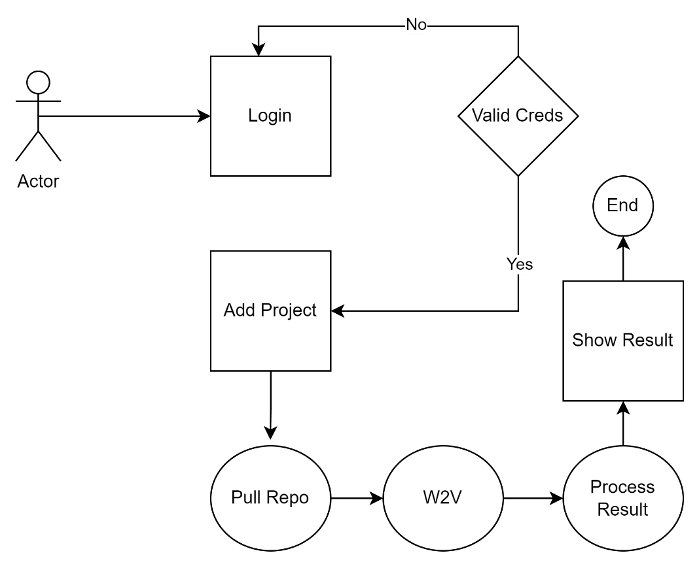
\includegraphics[width=0.9\linewidth]{images/workflow.png}
    \caption{SafeScript workflow diagram}
    \label{fig:workflow}
\end{figure}

This structured approach ensures that the system not only identifies security vulnerabilities effectively but also facilitates continuous improvement 
in code security through iterative scans and fixes.